\documentclass[a4paper,10pt]{article}
\usepackage[utf8]{inputenc}
\usepackage[UKenglish]{babel}
\usepackage{fancyhdr}
\usepackage{anysize}
\usepackage{amsmath, amsthm, amssymb}
\usepackage{lastpage}
\usepackage[all]{xy}  % drawings
%\usepackage{listings} % code highlighting
\usepackage[usenames,dvipsnames]{color}
\usepackage{graphicx}
\usepackage{caption}
\usepackage{subfigure}
\usepackage{hyperref}
\usepackage{framed,color}
\definecolor{shadecolor}{rgb}{0.8,0.8,0.8}
\usepackage{textcomp}

\pagestyle{fancy}
\fancyfoot[R]{\em \thepage / \pageref{LastPage}}
\fancyfoot[C]{}
\fancyfoot[L]{\em Master VIBOT}
\fancyhead[R]{\em Lab1 - Introduction to Turtlebot}
\fancyhead[C]{}
\fancyhead[L]{\em Probabilistic Robotics}
\renewcommand{\headrulewidth}{0.4pt}
\renewcommand{\footrulewidth}{0.4pt}


%\,	 a small space
%\:	 a medium space
%\;	 a large space
%\quad	 a really large space
%\qquad	 a huge space
%\!	 a negative space (moves things back to the left)
        
\begin{document}

\marginsize{2cm}{2cm}{2cm}{2cm}

% Title
%\hspace{1mm}
\begin{center}
\Large \textbf{Lab1 - Introduction to Turtlebot}
\end{center}
%\hspace{1mm}

\section{Introduction}

This lab is designed to do a first approach to the Turtlebot 2 \ref{fig:turtlebot2} and to get use to the ROS network configuration. This robot will be used in the upcoming lab sessions. You can find all the information related to this robot in \url{http://wiki.ros.org/Robots/TurtleBot}. Furthermore, this lab session is also an introduction to the ros launch system known as launch files.

\begin{figure}[h!]
	\centering
	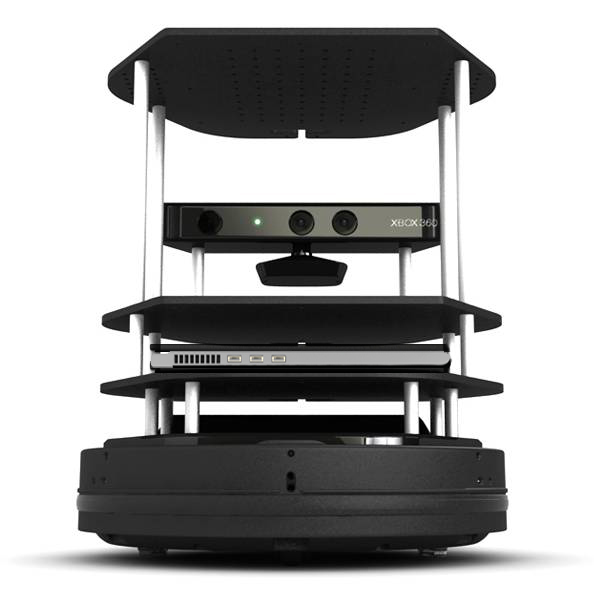
\includegraphics[width=3cm]{turtlebot2}
	\caption{Turtlebot 2 with a Kubuki base}
	\label{fig:turtlebot2}
\end{figure}


\section{Pre-lab}

Upgrade to hydro or indigo your ROS distribution (if you have newer versions the turtlebot packages are not available) following the instructions from \url{http://wiki.ros.org/hydro/Installation/Ubuntu}. We recommend to install the \texttt{ros-hydro-desktop-full} package. Furthermore, you need to install all the required Turtlebot packages by using \texttt{sudo apt-get install ros-hydro-turtlebot*} (only for hydro and indigo distribution). It is also recommended to install chrony \texttt{sudo apt-get install chrony} and synchronize the computer \texttt{sudo ntpdate ntp.ubuntu.com}. If your ROS distribution is Jade, you can do the pre-lab in the laboratory at the beginning using the virtual machines available.

After installing the hydro version and all the Turtlebot 2 packages follow this instructions:
\begin{itemize}
	\item Run \textit{roslaunch turtlebot\_gazebo turtlebot\_empty\_world.launch}. This package is the one that starts the robot simulation within the Gazebo simulator. If you are using indigo distribution use \textit{turtlebot\_world.launch}
	\item Add the Willow garage model to the gazebo simulator (place it so the robot is inside the building). You will have the model available after a while in the insert tab.
	\item Run \textit{roslaunch turtlebot\_teleop keyboard\_teleop.launch} in a new terminal. Drive the robot around using the keys indicated in the terminal.
	\item Run \textit{roslaunch turtlebot\_gazebo gmapping\_demo.launch} and \textit{roslaunch turtlebot\_rviz\_launchers \\ view\_navigation.launch} in two new terminals. Drive the robot around and build a map. Save a screen shot of Rviz where a map of at least two rooms can be seen (the visualizer, not the simulator) and submit it through the Moodle before the day of the lab.
\end{itemize}

\section{Lab work}
Most of the work asked here is based on the Turtlebot tutorials from \url{http://wiki.ros.org/Robots/TurtleBot}. For the robots use \textit{turtlebot} as user name and \textit{ros} as password.

\subsection{Network configuration}
In ROS, two main variables have to be set up before start working: the \texttt{ROS\_MASTER\_URI}, which tells the system which robot/computer will host the roscore, and the \texttt{ROS\_HOSTNAME}, which hosts the pc's IP or name. Pay special attention to this two variables if the messages are not properly sent or received over the network. If this happens, it means that the network configuration is wrong and some of the variables can not be resolved to an IP address.

\subsubsection{Working with your own computer}
In order to set up the network, connect to the appropriate wifi according to the robot (see table \ref{tab:ips}). Then, configure your network according to the IPs from table \ref{tab:ips}. For the configuration, three steps are done. First add the Turtlebot to the hosts file in \textit{/etc/hosts}: 
\begin{shaded}
	\begin{itemize}
		\item[\$] sudo sh -c \textquotesingle echo TURLEBOT\_IP  ROBOT\_NAME $>>$ /etc/hosts\textquotesingle
	\end{itemize}
\end{shaded}
Use the TURTLEBOT\_IP and ROBOT\_NAME from the following table:

\begin{table}[h!]
	\centering
	\begin{tabular}{|c|c|c|c|}
		\hline
		Robot Name & WiFi & Password & Robot's IP \\ \hline
		turtlebot1 & turtlebot1 & turtlebot1 & 10.42.0.1 \\ \hline
		turtlebot2 & turtlebot2 & turtlebot2 & 10.42.0.1 \\ \hline
		turtlebot3 & WLAN\_24 & C001D201E7A24 & 192.168.1.3 \\ \hline
		turtlebot4 & WLAN\_24 & C001D201E7A24 & 192.168.1.4 \\ \hline
		turtlebot5 & WLAN\_24 & C001D201E7A24 & 192.168.1.5 \\ \hline
	\end{tabular}
    \caption{Network configuration for Turtlebots. }
    \label{tab:ips}
\end{table}
and your computer's IP for YOUR\_IP. Then, set up your \texttt{ROS\_MASTER\_URI}:
\begin{shaded}
	\begin{itemize}
		\item[\$] echo export ROS\_MASTER\_URI=http://ROBOT\_NAME:11311 $>>$ /home/\$(whoami)/.bashrc
	\end{itemize}
\end{shaded}
finally set up your \texttt{ROS\_HOSTNAME}:
\begin{shaded}
	\begin{itemize}
		\item[\$] echo export ROS\_HOSTNAME=YOUR\_IP $>>$ /home/\$(whoami)/.bashrc
	\end{itemize}
\end{shaded}
For all this changes to take effect you have to reload your \texttt{.bashrc} file:
\begin{shaded}
	\begin{itemize}
		\item[\$] source /home/\$(whoami)/.bashrc
	\end{itemize}
\end{shaded}

To check if the connection is properly done, first we open an ssh connection to the robot:
\begin{shaded}
	\begin{itemize}
		\item[\$] ssh turtlebot@ROBOT\_NAME
	\end{itemize}
\end{shaded}
and there, we run a roscore. Then run in your pc's terminal:
\begin{shaded}
	\begin{itemize}
		\item[\$] rostopic list
	\end{itemize}
\end{shaded}
This command should return a list of topics if a the ROS master has a core running. If the ROS core is running in the master, and the \texttt{rostopic list} does not connects to it, the network configuration is not well done.

\subsubsection{Working with the computers from the laboratory}
To connect to the robots from the computers in the laboratory you have to connect your windows machine to the appropriate WiFi network \ref{tab:ips}. Switch on the virtual machine and connect the first network (Intel 82540EM Gigabit Ehternet Controller) to the appropriate turtlebot network and the second network interface (Red Hat Virtio network device) to internet\_acess to be able to surf the web.

To check if the connection is properly done, first we open an ssh connection to the robot:
\begin{shaded}
	\begin{itemize}
		\item[\$] ssh ROBOT\_NAME
	\end{itemize}
\end{shaded}
where ROBOT\_NAME is \texttt{turtlebot\#} (example: turtlebot1). There, we run a roscore. To set up the desktop terminal to work with that specific turtlebot type:
\begin{shaded}
	\begin{itemize}
		\item[\$] turtlebot\#
	\end{itemize}
\end{shaded}
where \# is the number of the turtlebot you are going to use. This will change your \texttt{ROS\_MASTER\_URI} to the specified robot. Finally on the desktop run:
\begin{shaded}
	\begin{itemize}
		\item[\$] rostopic list
	\end{itemize}
\end{shaded}
This command should return a list of topics if a the ROS master has a core running.

\subsection{Bringup}
In order to start the robot, ssh into it's computer and run:
\begin{shaded}
	\begin{itemize}
		\item[\$] roslaunch turtlebot\_bringup minimal.launch
	\end{itemize}
\end{shaded}
and, in your pc's terminal run:
\begin{shaded}
	\begin{itemize}
		\item[\$] roslaunch turtlebot\_dashboard turtlebot\_dashboard.launch
	\end{itemize}
\end{shaded}
This will launch a graphical interface to check the robot's status. Here you can check, among other things, the batteries of both the robot and its pc.

To start the Kinect on the robot run:
\begin{shaded}
	\begin{itemize}
		\item[\$] roslaunch turtlebot\_bringup 3dsensor.launch
	\end{itemize}
\end{shaded}
and, in a new terminal:
\begin{shaded}
	\begin{itemize}
		\item[\$] roslaunch turtlebot\_rviz\_launchers view\_robot.launch
	\end{itemize}
\end{shaded}
Note that if you want to visualize the data on your workstation the process will be very slow due to the amount of information to send through network. It is highly recommended to run this two commands directly on the turtlebot's pc, not via ssh.

\subsection{Teleoperation}
For the keyboard teleoperation ssh into the turtlebot and run:
\begin{shaded}
	\begin{itemize}
		\item[\$] roslaunch turtlebot\_teleop keyboard\_teleop.launch
	\end{itemize}
\end{shaded}

\subsection{Navigation and mapping}
This robot has already built up packages which allow to build maps using SLAM and also to do autonomous navigation on a given map. First, we are going to use the mapping node to obtain a small map. After bringing up the turtlebot and setting up the keyboard teleoperation, run (in a new terminal):
\begin{shaded}
	\begin{itemize}
		\item[\$] roslaunch turtlebot\_navigation gmapping\_demo.launch
	\end{itemize}
\end{shaded}
In order to visualize the map and the robot's position run:
\begin{shaded}
	\begin{itemize}
		\item[\$] roslaunch turtlebot\_rviz\_launchers view\_navigation.launch
	\end{itemize}
\end{shaded}
Drive the robot around to build a small map and capture a screen shot for the report. To save the map use, on the robot's pc:
\begin{shaded}
	\begin{itemize}
		\item[\$] rosrun map\_server map\_saver -f /tmp/my\_map
	\end{itemize}
\end{shaded}

In order to navigate the robot autonomously on that map launch (on the robot):
\begin{shaded}
	\begin{itemize}
		\item[\$] roslaunch turtlebot\_navigation amcl\_demo.launch map\_file:=/tmp/my\_map.yaml
	\end{itemize}
\end{shaded}
and close the teleoperation. If you have closed Rviz on your workstation use the same command as for the mapping to open it again. Now click on "2D Pose Estimate" and click where the robot is within the map (click for the position, and point for the direction). Now tell the robot where to go using "2D Nav Goal". Capture the screen while the robot is computing the trajectory for the report.

\subsection{Follower}
The last tutorials are two funny function for Turtlebot: the follower package and the panorama one. For the follower, run (on the robot):
\begin{shaded}
	\begin{itemize}
		\item[\$] roslaunch turtlebot\_follower follower.launch
	\end{itemize}
\end{shaded}
Now stand in front of the robot and move, it should follow you if you are not moving fast.

For the panorama package run (on the robot):
\begin{shaded}
	\begin{itemize}
		\item[\$] roslaunch turtlebot\_panorama panorama.launch
	\end{itemize}
\end{shaded}
now you can start the panorama by publishing the following:
\begin{shaded}
	\begin{itemize}
		\item[\$] rostopic pub turtlebot\_panorama/take\_pano std\_msgs/Empty
	\end{itemize}
\end{shaded}
or calling the following service:
\begin{shaded}
	\begin{itemize}
		\item[\$] rosservice call turtlebot\_panorama/take\_pano 0 360.0 30.0 0.3
	\end{itemize}
\end{shaded}
it can also be stopped using either one of the following calls:
\begin{shaded}
	\begin{itemize}
		\item[\$] rostopic pub turtlebot\_panorama/stop\_pano std\_msgs/Empty
		\item[\$] rosservice call turtlebot\_panorama/take\_pano 2 360.0 30.0 0.3
	\end{itemize}
\end{shaded}
capture a panorama for the report. To view the panorama run:
\begin{shaded}
	\begin{itemize}
		\item[\$] rosrun image\_view image\_view image:=/turtlebot\_panorama/panorama
	\end{itemize}
\end{shaded}

\subsection{Turtlebot driver}
Along with the lab documentation you can find a ROS package called \texttt{lab1\_turtlebot}. This package contains the script where the lab programming will be done. Please modify the driver.py (\texttt{lab1\_turtlebot/src/driver.py}) in order to be able to make the Turtlebot go to a given position. For this purpose, please modify the constructor of the driver class where the definition of the subscriber, publisher and velocity message are missing. You will have to modify also the functions \texttt{read\_position}, which stores the position received on a message to the class variables, and \texttt{compute\_velocity} where the velocity message is created.

To launch the node run:
\begin{shaded}
	\begin{itemize}
		\item[\$] roslaunch lab1\_turtlebot driver.launch
	\end{itemize}
\end{shaded}
If no arguments are given to the \texttt{driver.lanch}, the goal point is $(0,0,0)$ for $(x,y,\theta)$. If you want this points to change use:
\begin{shaded}
	\begin{itemize}
		\item[\$] roslaunch lab1\_turtlebot driver.launch x:=$x$ y:=$y$ theta:=$\theta$
	\end{itemize}
\end{shaded}
Furthermore, it is possible to launch this node in a virtual environment. For this purpose first you have to set up your masters to your workstation to avoid problems with the real robot:
\begin{shaded}
	\begin{itemize}
		\item[\$] export ROS\_MASTER\_URI=http://localhost:11311
	\end{itemize}
\end{shaded}
(the laboratory desktops have a short cut by typing \texttt{local} in the terminal you want it to have itself as \texttt{ROS\_MASTER\_URI}) now, the terminal where you have run this command uses your workstation as ROS master. To launch the simulator run:
\begin{shaded}
	\begin{itemize}
		\item[\$] roslaunch turtlebot\_driver driver.launch sim:=true
	\end{itemize}
\end{shaded}
Please note that the this parameter can be combined with the previous ones to set up a goal location.


\section{Optional}

Modify you \texttt{turtlebot\_driver.py} in order to be able to read from a txt file (given as input for the launch file) a whole trajectory instead of just going to one point. In this case you will have to modify also the function \texttt{load\_goals} and \texttt{next\_goal}. The trajectory file will have the following structure:
\begin{shaded}
	\begin{itemize}
		\item[] $x_0$,$y_0$,$\theta_0$
		\item[] $x_1$,$y_1$,$\theta_1$
		\item[] . . .
		\item[] $x_n$,$y_n$,$\theta_n$
	\end{itemize}
\end{shaded}
and will be passed as an argument called \texttt{file} to the launch file. Please find an example of a trajectory in \texttt{others/list.txt}

\section{Lab report}

Upload a zip file containing the report (2-3 pages in pdf format) as well as the final \texttt{driver.py} file. If you have done the optional part, please submit the new launch file also.

\end{document}
